% Section content template for individual Educative lessons
% This file contains the actual content for a specific section
% Generated from Educative API section content

% Section: Evaluation of a Distributed Search's Design
% Section ID: 4962799423324160
% Section Slug: evaluation-of-a-distributed-searchs-design
% Generated: 2025-12-07T21:52:28.407293

\subsection{Requirements compliance}\label{_sb-_cCbIB_-wveiRJU9A}
\\
Let's discuss how our proposed design of a distributed search fulfills the non-functional requirements.

\subsubsection{Availability}\label{cWeRoe4bMVy-4c80Zi8Q1}
\\
We utilized distributed storage to store these items:

\begin{itemize}
\item
\protect\phantomsection\label{pv00IRde78aqPIXBatl7U}
Documents crawled by the indexer.
\item
\protect\phantomsection\label{MtEzEckuMEcdTMGQfGoOo}
Inverted indexes generated by the indexing nodes.
\end{itemize}
\\
Data is replicated across multiple regions in distributed storage, making cross-region deployment for indexing and search easier. The group of indexing and search nodes merely needs to be replicated in different availability zones. Therefore, we deploy the cluster of indexing and search nodes in different availability zones. So , if a failure occurs in one place, we can process the requests from another cluster. Multiple groups of indexing and search nodes help to achieve high indexing and search availability. Moreover
, in each cluster, if a node dies, another can take its place.
\\
The indexing is performed offline, not on the user's critical path. We don't need to replicate the indexing operations synchronously. It is unnecessary to respond to the user search queries with the latest data that has just been added to the index. So , we don't have to wait for the replication of the new index to respond to the search queries. This makes the search available to the users.
\begin{quote}
\textbf{Note:} Once we replicate the latest data in all groups of indexing nodes and the search nodes have downloaded it, then the search queries are performed on the latest data.
\end{quote}

\begin{figure}[htbp]
 \centering
 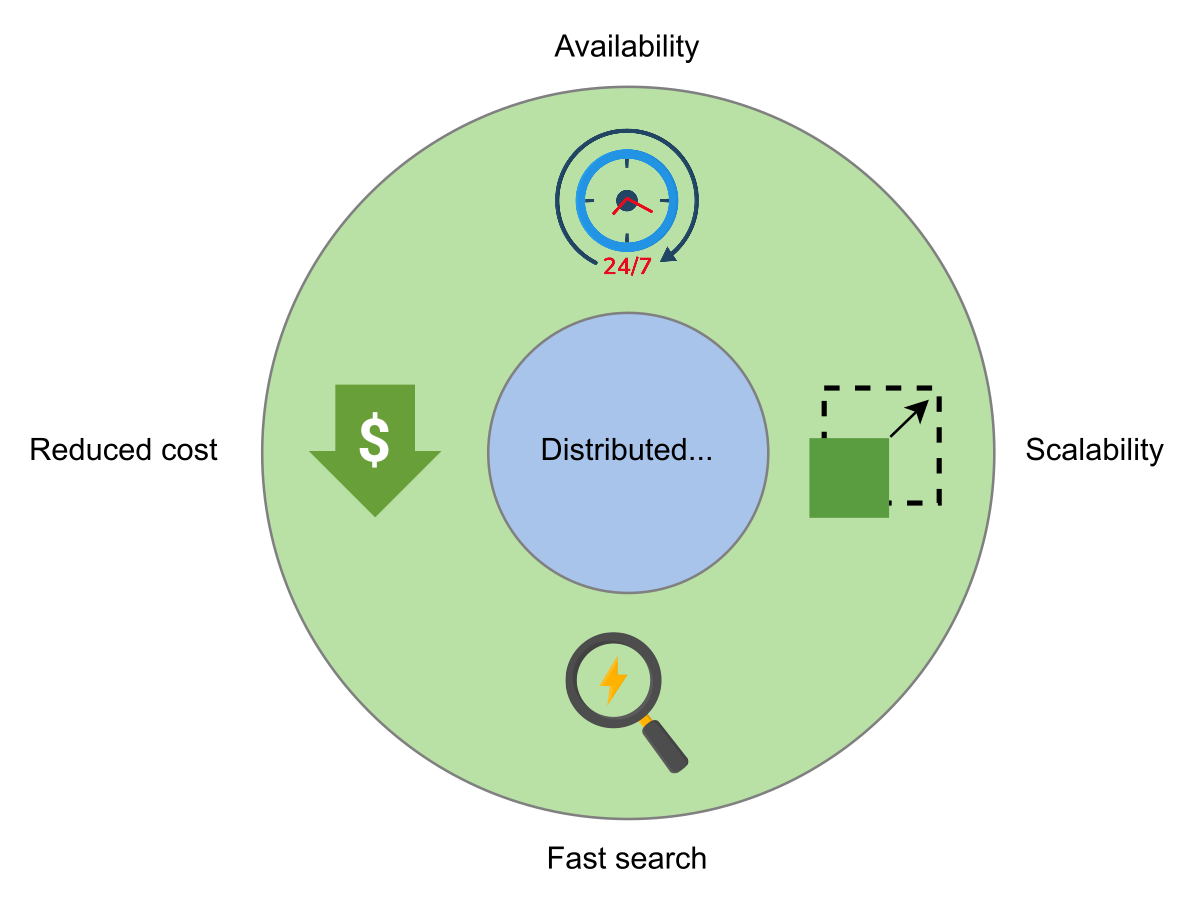
\includegraphics[width=0.5\textwidth]{Images/chapter_21/section_4962799423324160/6633442511159296.png}
 \caption{Guarantees provided by the distributed search}
\end{figure}

\subsubsection{Scalability}\label{ZU6EnBEUsLkdQ33umfDHW}
\\
\hfill\break
Partitioning is an essential component of search systems to scale. When we increase the number of partitions and add more nodes to the indexing and search clusters, we can scale in terms of data indexing and querying.\\
\strut \\
The strong isolation of indexing and search processes help indexing and search scale independently and dynamically.
\\
You're a software engineer for a rapidly growing e-commerce site aiming to redefine search with lightning-fast personalized results. Currently , user experience is suffering due to slow search response times, especially during peak loads.
\\
Your task is to:

\begin{itemize}
\item
Identify components of distributed search that can benefit from caching to improve performance.
\item
Identify the potential trade-offs to consider.
\end{itemize}
\\

\subsubsection{Fast search on big data}\label{FBdLknxK9DdAmqCH0-0O_}
\\
We utilized a number of nodes, each of which performs search queries in parallel on smaller inverted indices. The result from each search node is then merged and returned to the user.

\subsubsection{Reduced cost}\label{xNVHGT97AjetXx5sRmbn0}
\\
We used cheaper machines to compute indexes and perform searches. If one node fails, we don't have to recompute the complete index. Instead, some of the documents need to be indexed again.

\subsection{Conclusion}\label{sYkJZPI4j5U3ZyQr-xKCe}
\\
A search system is required for almost every application. We have seen that it isn't possible to develop a search system that can run on a single node. We utilized a parallel computation framework and low-cost machines to build a search system that is available, scalable, and highly performant.

% End of section content